\documentclass[12pt,convert={false}]{standalone}
\usepackage[dvipsnames]{xcolor}
\usepackage{tikz}
\usetikzlibrary{shapes,arrows,positioning,calc,patterns,arrows.meta, bending, graphs, shadings,quotes,intersections}
\usetikzlibrary{external}
%\tikzexternalize[prefix=tikz/]
\usepackage{pgfplots}
\pgfplotsset{compat=1.16}
\usepgfplotslibrary{fillbetween}
\newcommand{\enf}[1]{\textcolor{RedViolet}{\textbf{#1}}} %enf sta per enfasi
\newcommand{\sott}[1]{\setulcolor{black!20!Goldenrod}\ul{#1}}
\newcommand{\prob}{\mathbb{P}}
\newcommand\independent{\protect\mathpalette{\protect\independenT}{\perp}}
\newcommand{\ev}[1]{\mathbb{E}\Bigl[{#1}\Bigr]}
\def\independenT#1#2{\mathrel{\rlap{$#1#2$}\mkern2mu{#1#2}}}
\newcommand{\Z}{\mathbb{Z}}
\newcommand{\R}{\mathbb{R}}
\newcommand{\N}{\mathbb{N}}
\newcommand{\equalexpl}[1]{%
	\underset{\substack{\uparrow\\\mathrlap{\text{\vspace{-3cm}\hspace{-1em}#1}}}}{=}}
\newcommand{\dif}{\mathop{}\!\mathrm{d}}
\begin{document}

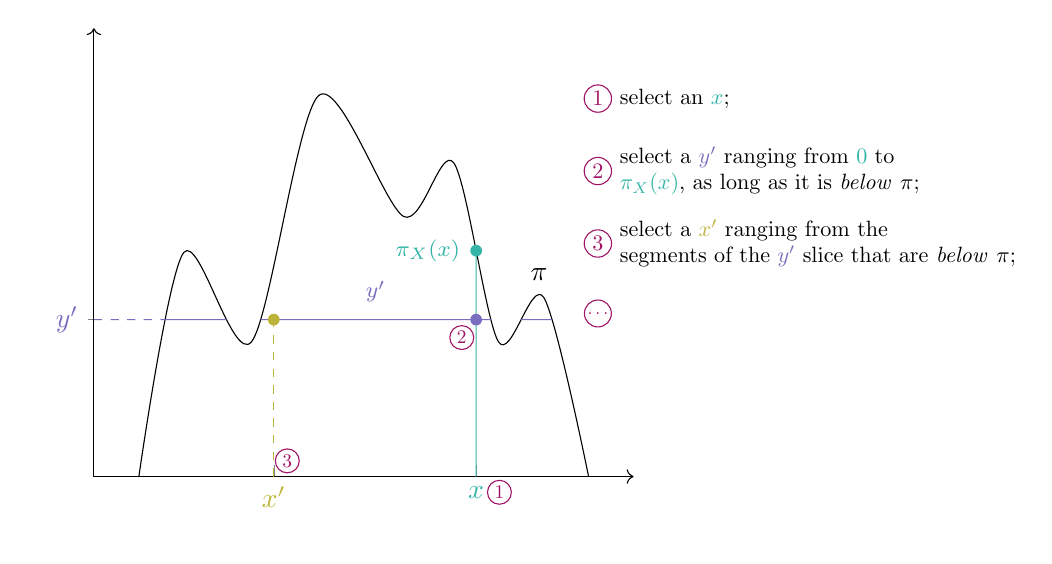
\begin{tikzpicture}[every label/.style={align=left}]
	\begin{axis}[
		xlabel=\empty,
		xtick={400,850},
		xticklabels={\textcolor{yellow!70!black}{$x'$},\textcolor{Turquoise!80!black}{$x$}},
		x axis line style={->,opacity=100},
		ytick={35},
		yticklabels={\textcolor{Periwinkle}{$y'$}},
		ylabel=\empty,
		xmin=0, xmax=1200,
		ymin=0, ymax=100,
		axis y line=left,
		y axis line style={->,opacity=100},
		axis x line*=bottom
		]
		\addplot[smooth,name path=A] coordinates {
			(100,0)
			(200,50)
			(350,30)
			(500,85)
			(689,58)
			(800,70)
			(900,30)
			(1000,40)
			(1100,0)
		};
		\node[align=left] at (990,45) {$\pi$};
		\path[name path=vert1](850,0)--(850,100);
		\fill [name intersections={of=A and vert1}] (intersection-1) coordinate (a) node[circle,fill,Turquoise!80!black,inner sep=1.5pt,label=left:\textcolor{Turquoise!80!black}{\footnotesize$\pi_X(x)$}]{};
		\draw[Turquoise!80!black] (850,0) -- (a);
		\path[name path=hor1](0,35)--(1200,35);
		\fill [name intersections={of=A and hor1}] 
		(intersection-1) coordinate (b) 
		(intersection-2) coordinate (c) 
		(intersection-3) coordinate (d)
		(intersection-4) coordinate (e)
		(intersection-5) coordinate (f)
		(intersection-6) coordinate (g)
		;
		\draw[Periwinkle](b)--(c);
		\draw[Periwinkle](d)--(e) node[circle,midway,above]{\footnotesize$y'$};
		\draw[Periwinkle](f)--(g);
		\draw[Periwinkle,dashed](0,35)--(b);
		\fill[name intersections={of=vert1 and hor1}] (intersection-1) node[circle,fill,Periwinkle,inner sep=1.5pt]{};
		\draw[yellow!70!black,dashed](400,0)--(400,35) node[circle,fill,inner sep=1.5pt]{};
		\node[circle,draw,RedViolet,inner sep=1.5pt,scale=0.7]at(818,31){2};
		\node[circle,draw,RedViolet,inner sep=1.5pt,scale=0.7]at(430,3.5){3};
	\end{axis}
	\node[circle,draw,RedViolet,inner sep=1.5pt,scale=0.7]at(5.15,-0.2){1};
	\begin{scope}[scale=0.8, every node/.append style={transform shape}]
		\node[circle,draw,RedViolet,inner sep=1.5pt,scale=1,label=right:{select an \textcolor{Turquoise!80!black}{$x$};}](lol) at(8,6){1};
		\node[circle,draw,RedViolet,inner sep=1.5pt,scale=1,label=right:{select a \textcolor{Periwinkle}{$y'$} ranging from \textcolor{Turquoise!80!black}{0} to\\ \textcolor{Turquoise!80!black}{$\pi_X(x)$}, as long as it is \textit{below} $\pi$;}](lmao)[below=20pt of lol]{2};
		\node[circle,draw,RedViolet,inner sep=1.5pt,scale=1,label=right:{select a \textcolor{yellow!70!black}{$x'$} ranging from the \\segments of the \textcolor{Periwinkle}{$y'$} slice that are \textit{below} $\pi$;}](kek)[below=20pt of lmao]{3}; 
		\node[circle,draw,RedViolet,inner sep=1.5pt,scale=0.8,label=right:{}](dotz)[below=19pt of kek]{$\ldots$};
	\end{scope}
\end{tikzpicture}
\end{document}
